% Alternate prose version. Shares the verified numerical assets and official style.
% The primary manuscript and submission archives are separate from this version.
\documentclass{article}
\usepackage{neurips_2026}
\usepackage[utf8]{inputenc}
\usepackage[T1]{fontenc}
\usepackage{hyperref}
\usepackage{url}
\usepackage{booktabs}
\usepackage{amsmath,amssymb,amsfonts}
\usepackage{microtype}
\usepackage{graphicx}
\graphicspath{{figures/}}
% Generated by analysis/build_submission_assets.py; do not edit.
\newcommand{\RawSmallTen}{0.276}
\newcommand{\MagnitudeSmallTen}{0.411}
\newcommand{\DiagonalSmallTen}{0.786}
\newcommand{\PoissonSmallTen}{1.000}
\newcommand{\AMGSmallTen}{0.986}
\newcommand{\EnergySmallTen}{0.766}
\newcommand{\RawSmallHundred}{0.244}
\newcommand{\MagnitudeSmallHundred}{0.448}
\newcommand{\DiagonalSmallHundred}{0.681}
\newcommand{\PoissonSmallHundred}{1.000}
\newcommand{\AMGSmallHundred}{0.920}
\newcommand{\EnergySmallHundred}{0.788}
\newcommand{\RawSmallFiveHundred}{0.214}
\newcommand{\MagnitudeSmallFiveHundred}{0.441}
\newcommand{\DiagonalSmallFiveHundred}{0.670}
\newcommand{\PoissonSmallFiveHundred}{0.999}
\newcommand{\AMGSmallFiveHundred}{0.867}
\newcommand{\EnergySmallFiveHundred}{0.791}
\newcommand{\RawLargeTen}{0.165}
\newcommand{\MagnitudeLargeTen}{0.391}
\newcommand{\DiagonalLargeTen}{0.552}
\newcommand{\PoissonLargeTen}{1.000}
\newcommand{\AMGLargeTen}{0.972}
\newcommand{\EnergyLargeTen}{0.714}
\newcommand{\RawLargeHundred}{0.152}
\newcommand{\MagnitudeLargeHundred}{0.438}
\newcommand{\DiagonalLargeHundred}{0.550}
\newcommand{\PoissonLargeHundred}{1.000}
\newcommand{\AMGLargeHundred}{0.884}
\newcommand{\EnergyLargeHundred}{0.728}
\newcommand{\RawLargeFiveHundred}{0.118}
\newcommand{\MagnitudeLargeFiveHundred}{0.437}
\newcommand{\DiagonalLargeFiveHundred}{0.561}
\newcommand{\PoissonLargeFiveHundred}{0.999}
\newcommand{\AMGLargeFiveHundred}{0.831}
\newcommand{\EnergyLargeFiveHundred}{0.731}
\newcommand{\RecallSmallHundredTwenty}{62.5}
\newcommand{\RecallSmallHundredTwentyLow}{58.4}
\newcommand{\RecallSmallHundredTwentyHigh}{66.7}
\newcommand{\RecallSmallHundredForty}{100.0}
\newcommand{\RecallSmallHundredFortyLow}{100.0}
\newcommand{\RecallSmallHundredFortyHigh}{100.0}
\newcommand{\RecallSmallFiveHundredTwenty}{18.7}
\newcommand{\RecallSmallFiveHundredTwentyLow}{15.0}
\newcommand{\RecallSmallFiveHundredTwentyHigh}{22.7}
\newcommand{\RecallSmallFiveHundredForty}{99.5}
\newcommand{\RecallSmallFiveHundredFortyLow}{99.3}
\newcommand{\RecallSmallFiveHundredFortyHigh}{99.7}
\newcommand{\RecallLargeHundredTwenty}{50.8}
\newcommand{\RecallLargeHundredTwentyLow}{46.3}
\newcommand{\RecallLargeHundredTwentyHigh}{55.2}
\newcommand{\RecallLargeHundredForty}{100.0}
\newcommand{\RecallLargeHundredFortyLow}{100.0}
\newcommand{\RecallLargeHundredFortyHigh}{100.0}
\newcommand{\RecallLargeFiveHundredTwenty}{10.9}
\newcommand{\RecallLargeFiveHundredTwentyLow}{8.0}
\newcommand{\RecallLargeFiveHundredTwentyHigh}{13.9}
\newcommand{\RecallLargeFiveHundredForty}{98.7}
\newcommand{\RecallLargeFiveHundredFortyLow}{98.4}
\newcommand{\RecallLargeFiveHundredFortyHigh}{99.0}
\newcommand{\PoissonLargeFiveHundredPrecise}{0.9985}
\newcommand{\PoissonCorrectionRemainingPercent}{1.29}
\newcommand{\PoissonTopOverlapPercent}{99.15}
\newcommand{\PoissonTopOverlapPercentLow}{98.91}
\newcommand{\PoissonTopOverlapPercentHigh}{99.34}
\newcommand{\PredictionRelativePercentTen}{3.45}
\newcommand{\PredictionRelativePercentHundred}{10.54}
\newcommand{\PredictionRelativePercentFiveHundred}{13.53}
\newcommand{\FluxRecallLargeFiveHundredTwenty}{16.3}
\newcommand{\FluxRecallLargeFiveHundredTwentyLow}{12.9}
\newcommand{\FluxRecallLargeFiveHundredTwentyHigh}{20.0}
\newcommand{\FluxRecallLargeFiveHundredForty}{99.3}
\newcommand{\FluxRecallLargeFiveHundredFortyLow}{99.1}
\newcommand{\FluxRecallLargeFiveHundredFortyHigh}{99.5}
\newcommand{\PoissonTimeSmall}{0.770}
\newcommand{\PoissonTimeSmallLow}{0.767}
\newcommand{\PoissonTimeSmallHigh}{0.778}
\newcommand{\AdaptiveTimeSmall}{1.572}
\newcommand{\AdaptiveTimeSmallLow}{1.426}
\newcommand{\AdaptiveTimeSmallHigh}{1.753}
\newcommand{\AMGTimeSmall}{3.184}
\newcommand{\AMGTimeSmallLow}{3.151}
\newcommand{\AMGTimeSmallHigh}{3.323}
\newcommand{\FluxAdaptiveTimeRatioSmall}{1.152}
\newcommand{\PoissonTimeLarge}{0.325}
\newcommand{\PoissonTimeLargeLow}{0.319}
\newcommand{\PoissonTimeLargeHigh}{0.328}
\newcommand{\AdaptiveTimeLarge}{0.736}
\newcommand{\AdaptiveTimeLargeLow}{0.678}
\newcommand{\AdaptiveTimeLargeHigh}{0.753}
\newcommand{\AMGTimeLarge}{1.345}
\newcommand{\AMGTimeLargeLow}{1.315}
\newcommand{\AMGTimeLargeHigh}{1.395}
\newcommand{\FluxAdaptiveTimeRatioLarge}{1.116}
\newcommand{\AdaptiveIterationsLargeFiveHundred}{33.5}
\newcommand{\FluxAdaptiveIterationsLargeFiveHundred}{32.1}
\newcommand{\LongtrainRelativeLTwoPercent}{9.03}
\newcommand{\LongtrainRawRho}{0.223}
\newcommand{\UnetRelativeLTwoPercent}{4.41}
\newcommand{\UnetRawRho}{0.231}

% Generated from results/smooth_robustness/summary.json.
\newcommand{\SmoothCorrectionRemainingPercent}{0.59}
\newcommand{\SmoothCorrectionRemainingPercentHigh}{0.63}
\newcommand{\SmoothCorrectionRemainingPercentLow}{0.56}
\newcommand{\SmoothFluxRecallPercent}{36.5}
\newcommand{\SmoothFluxRecallPercentHigh}{39.1}
\newcommand{\SmoothFluxRecallPercentLow}{33.9}
\newcommand{\SmoothPairedRhoGain}{1.041}
\newcommand{\SmoothPairedRhoGainHigh}{1.062}
\newcommand{\SmoothPairedRhoGainLow}{1.020}
\newcommand{\SmoothPoissonRho}{0.9999}
\newcommand{\SmoothPoissonRhoHigh}{0.9999}
\newcommand{\SmoothPoissonRhoLow}{0.9999}
\newcommand{\SmoothRawRho}{-0.041}
\newcommand{\SmoothRawRhoHigh}{-0.020}
\newcommand{\SmoothRawRhoLow}{-0.062}
\newcommand{\SmoothRelativePercent}{4.13}
\newcommand{\SmoothRelativePercentHigh}{4.36}
\newcommand{\SmoothRelativePercentLow}{3.92}
\newcommand{\SmoothTopOverlapPercent}{99.5}
\newcommand{\SmoothTopOverlapPercentHigh}{99.6}
\newcommand{\SmoothTopOverlapPercentLow}{99.4}

\hypersetup{hidelinks,pdftitle={From PDE Residuals to Error Rankings in Elliptic Neural Operators},pdfauthor={}}
\title{From PDE Residuals to Error Rankings\\in Elliptic Neural Operators}
\author{Anonymous Author(s)}
\begin{document}
\maketitle

\begin{abstract}
A PDE residual checks whether a neural operator's prediction satisfies the equation. But does it
also show where the prediction is wrong? On elliptic problems across two grids and three binary
coefficient contrasts, and in a separately trained smooth-coefficient control, raw residual maps
locate pointwise error poorly, below simple prediction and geometry scores. Partial solves recover
much better error maps. In one challenging setting, estimated and true top-$10\%$ error sets
overlap by $\PoissonTopOverlapPercent\%$, yet a classical bound certifies only
$\FluxRecallLargeFiveHundredTwenty\%$ of the true set as members. Most of the prediction
correction is already computed by this stage. Checking the equation, ranking spatial errors and
certifying which cells have the largest errors are distinct tasks; moving between them has a solve cost.
\end{abstract}

\section{Introduction}
Neural operators learn to predict PDE solutions from data \citep{li2021fourier}. How can we assess a
new prediction without a reference solution? Substituting it into the equation gives a residual: a
check of equation consistency, which can itself be a target for uncertainty quantification
\citep{gopakumar2025calibratedphysicsinformeduncertaintyquantification}. Locating large prediction
errors asks more. A cell where the equation is poorly satisfied need not be a cell where the solution
error is large.

To see the distinction, consider the discrete problem $Au=b$. For a prediction $\hat u$, write
$e=\hat u-u$ for its error and $r=A\hat u-b$ for its residual. Then
\begin{equation}
 r=Ae,\qquad e=A^{-1}r.
 \label{eq:identity}
\end{equation}
For diffusion, the residual measures the divergence of an error flux. Nearby face contributions can
cancel, and their weights depend on the material coefficient. Its pattern therefore differs from the
error itself. Applying $A^{-1}$ recovers the error but requires another solve. A useful diagnostic must
balance the information it provides against this work.

The identity $e=A^{-1}r$ is classical. Our contribution is to measure what information about a
learned predictor's spatial error becomes available at intermediate solve budgets, before the
inverse is fully applied. We compare equation consistency, empirical ranking, certified top-error
membership and actual prediction correction. Our tools build on preconditioning and error estimation
\citep{li2020posteriorierrorestimatesfinite}, neural-operator residual correction
\citep{cao2022residualbasederrorcorrectionneural,jha2023residualbasederrorcorrectoroperator}, and
pointwise and equilibrated-flux bounds \citep{anwer2026pointwise,ern2011unified}. With simple
baselines, fresh fields and measured solve costs, we show that accurate rankings can support few
certified decisions while already computing most of the prediction correction.

\begin{figure}[t]
\centering
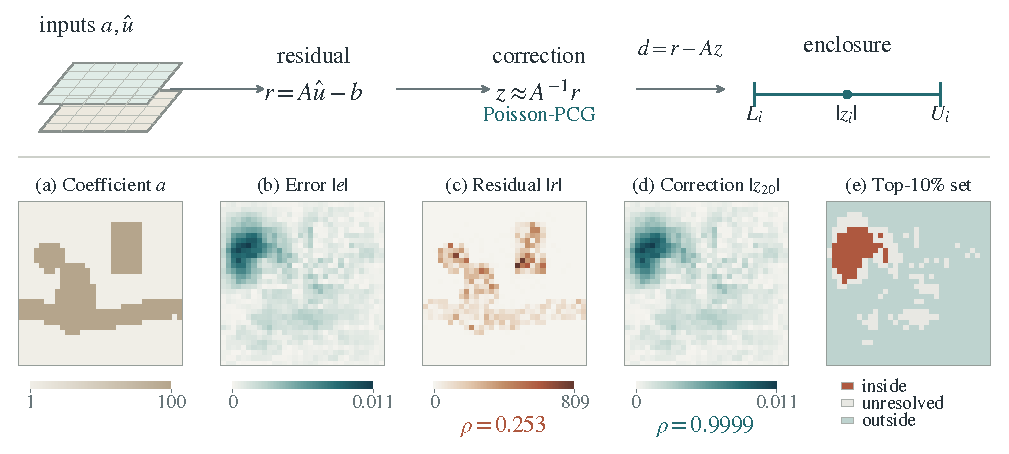
\includegraphics[width=\linewidth]{submission_maps_alternate.pdf}
\caption{Error maps and conservative decisions for one fresh $32^2$, $\kappa=100$ field, selected
by proximity to median raw-residual Spearman. Reference error $|e|$ is used only for evaluation and
shares a color scale with $|z_{20}|$. The flux bound identifies members and nonmembers of the
top-$10\%$ error set, leaving others unresolved. Aggregate results use all $200$ fields.}
\label{fig:maps}
\end{figure}

\section{Experimental setup}
\textbf{Problem and predictions.}
We solve $-\nabla\!\cdot(a\nabla u)=f$ on $[0,1]^2$, with zero Dirichlet boundary conditions and
$f(x,y)=1+0.25\sin(2\pi x)\sin(\pi y)$. The coefficient takes values $a\in\{1,\kappa\}$ in random
inclusions and channels; $\kappa\in\{10,100,500\}$ controls the contrast. We use $32^2$ and $64^2$
cell grids. A cell-centered two-point-flux discretization, with harmonic face coefficients and half-cell
boundary distances, gives a symmetric positive definite matrix $A$.

Each grid and contrast has a separate ensemble of three Fourier neural operators (FNOs): $700$
training fields, $80$ epochs, three layers, $12$ Fourier modes and $24$ channels per member.
Normalization uses training data only; $\hat u$ is the ensemble mean. After exploration on $200$
original test fields, we fixed methods and budgets, then drew $200$ fresh geometries matched across
contrasts and grids. Models remain frozen; resolutions are trained separately. Predictions use
float32; solves and diagnostics use float64. Eq.~\eqref{eq:identity} holds with the same $A$ to relative
tolerance $10^{-8}$ on every field. Bounds and training controls are subsequent exploratory checks;
optimization settings are in the artifact.

A matched smooth-family FNO check uses $32^2$, $\kappa=100$, the same forcing and training budget,
and independent $700/200$ train/test fields. We Gaussian-filter white noise (standard deviation
$0.12$ domain lengths), scale each field to $t\in[0,1]$, and set $a=100^t$. Comparisons with binary
media are descriptive: the coefficient distribution and trained predictor both change.

\textbf{Comparisons and measurements.}
Cheap scores are ensemble standard deviation, prediction magnitude $|\hat u|$, distance to the
nearest boundary, and residual magnitude $|r|$. Partial solves of $Az=r$ use $|z|$ to estimate spatial
error. We compare undamped Jacobi, conjugate gradients (CG), diagonal-PCG, and one full-hierarchy
smoothed-aggregation algebraic multigrid (AMG) V-cycle \citep{bell2023pyamg}. The Poisson matrix
$B=A(1)$ is inverted by an orthonormal discrete sine transform matched to the cell boundaries.
We use this inverse directly or as a CG preconditioner (Poisson-PCG). Iterations start from zero,
with budgets of $5,10,20,40,80$ steps.

We average spatial Spearman correlations with $|e|$ over fields. Percentile $95\%$ intervals use
$5{,}000$ field-bootstrap resamples, paired across methods and conditional on the frozen networks.
The top $10\%$ is a representative hotspot budget; ties are treated uniformly. We also compare
cell error energies: nonnegative face contributions, including boundaries, that sum to $e^TAe$.

\textbf{Turning an estimate into a decision.}
An error map alone does not justify each cell's ranking. We bound the error left after a correction
$z$, writing $d=r-Az$ and $a_{\min}=\min_i a_i$. Since $A\succeq a_{\min}B$ in quadratic-form
order, a classical pointwise bound \citep{anwer2026pointwise} gives
\begin{equation}
 |e_i-z_i|\le\beta_i
 :=\frac{\sqrt{(B^{-1})_{ii}\,d^TB^{-1}d}}{a_{\min}}.
 \label{eq:bound}
\end{equation}
Energy Cauchy--Schwarz and inverse ordering give this bound. It adds one Poisson solve, with
the inverse diagonal precomputed per grid; the artifact details the derivation and setup costs.

A tighter bound uses the actual face coefficients, following equilibrated-flux estimation
\citep{ern2011unified}. Write $A=DW_AD^T$ and $B=DW_BD^T$, with cell-face incidence $D$
and diagonal face weights, including boundaries. The Poisson flow $q=W_BD^TB^{-1}d$ satisfies
$Dq=d$ and bounds the remaining error energy by $E_{\rm eq}=q^TW_A^{-1}q$. This gives
\begin{equation}
 |e_i-z_i|\le\beta_i^{\rm eq}:=\sqrt{(B^{-1})_{ii}E_{\rm eq}/a_{\min}}\le\beta_i.
 \label{eq:fluxbound}
\end{equation}
This version reuses the Poisson solve and adds coefficient-weighted face sums.

Either bound, denoted by $\bar\beta_i$, gives an interval for the error magnitude:
$L_i=\max(|z_i|-\bar\beta_i,0)$ and $U_i=|z_i|+\bar\beta_i$. We certify a cell as belonging to the
largest-error set when its lower bound exceeds enough of the other upper bounds. Specifically,
for $m=\lceil0.1N^2\rceil$, it is certainly inside if $L_i>U_{(m+1)}$, and certainly outside if
$U_i<L_{(m)}$, with parentheses denoting descending order. Other cells remain unresolved; strict inequalities handle ties. These are exact-arithmetic implications
for the discrete problem, not interval-arithmetic guarantees for our float64 checks. Ground truth
only evaluates the decisions. An exploratory rule checks every five iterations, stopping at
$\lceil0.9m\rceil$ identified members or $80$ iterations. With valid bounds, reaching this target
guarantees $90\%$ top-set recall without a reference solution.

\section{Results}
\begin{table}[ht]
\centering
\caption{Mean spatial Spearman with $|e|$ on fresh $32^2$ binary fields, with $95\%$ field-bootstrap
intervals. Equal iterations are not equal work; $1.000$ denotes rounding, not exact recovery.}
\label{tab:localization}
% Generated from fresh32 summary; brackets are 95% field-bootstrap CIs.
\begin{tabular}{lccc}
\toprule
Score / correction & $\kappa=10$ & $\kappa=100$ & $\kappa=500$ \\
\midrule
raw $|r|$ & 0.276 [0.264, 0.289] & 0.244 [0.227, 0.261] & 0.214 [0.194, 0.233] \\
ensemble $\sigma$ & 0.238 [0.223, 0.253] & 0.318 [0.302, 0.333] & 0.327 [0.311, 0.343] \\
prediction $|\hat u|$ & 0.411 [0.385, 0.438] & 0.448 [0.425, 0.471] & 0.441 [0.417, 0.464] \\
boundary distance & 0.412 [0.387, 0.437] & 0.410 [0.388, 0.432] & 0.368 [0.344, 0.393] \\
Jacobi-20 & 0.489 [0.469, 0.508] & 0.508 [0.491, 0.524] & 0.531 [0.513, 0.550] \\
CG-20 & 0.551 [0.532, 0.569] & 0.355 [0.344, 0.368] & 0.278 [0.263, 0.293] \\
diagonal PCG-20 & 0.786 [0.768, 0.803] & 0.681 [0.658, 0.703] & 0.670 [0.646, 0.695] \\
$|B^{-1}r|$ & 0.613 [0.594, 0.632] & 0.408 [0.384, 0.431] & 0.355 [0.330, 0.381] \\
one AMG V-cycle & 0.986 [0.984, 0.987] & 0.920 [0.907, 0.932] & 0.867 [0.847, 0.885] \\
Poisson-PCG-20 & 1.000 [1.000, 1.000] & 1.000 [1.000, 1.000] & 0.999 [0.999, 1.000] \\
\bottomrule
\end{tabular}

\end{table}

\textbf{Residual maps miss much of the pointwise error pattern.}
As Table~\ref{tab:localization} shows, raw residuals give weak rankings, below even prediction
magnitude and distance to the boundary. They are more closely related to error energy. At $64^2$
and $\kappa=500$, for example, the mean residual correlation is $\RawLargeFiveHundred$ with
pointwise error and $\EnergyLargeFiveHundred$ with energy. This is an empirical finding, not a consequence of Eq.~\eqref{eq:identity} alone.

The mismatch persists with more accurate predictors (Table~\ref{tab:robustness}). Longer FNO
training and a U-Net ensemble \citep{ronneberger2015unet} reduce prediction error without improving
raw-residual ranking. The U-Net uses the same fields, three seeds, $200$ epochs and two levels
with $16/32/64$ channels.

\begin{table}[!htbp]
\centering
\caption{Controls at $32^2$, $\kappa=100$: means and $95\%$ field-bootstrap intervals on $200$
fields per row. The smooth FNO is separately trained; PCG-20 uses the Poisson preconditioner.}
\label{tab:robustness}
% Generated from independently verified retained ensemble summaries.
\begin{tabular}{@{}lccc@{}}
\toprule
Predictor (epochs) & Rel. $L^2$ error (\%) & Residual $\rho$ & PCG-20 $\rho$ \\
\midrule
Binary FNO (80) & 10.54 [9.44, 11.75] & 0.244 [0.227, 0.261] & 0.99998 [0.99998, 0.99999] \\
Binary FNO (240) & 9.03 [8.00, 10.16] & 0.223 [0.204, 0.240] & 0.99999 [0.99998, 0.99999] \\
Binary U-Net (200) & 4.41 [3.75, 5.15] & 0.231 [0.211, 0.250] & 0.99997 [0.99996, 0.99998] \\
Smooth FNO (80) & 4.13 [3.92, 4.36] & -0.041 [-0.062, -0.020] & 0.99994 [0.99994, 0.99995] \\
\bottomrule
\end{tabular}

\end{table}

The mismatch also occurs without binary interfaces (Table~\ref{tab:robustness}). For smooth fields,
twenty Poisson-PCG steps give top-set overlap of
$\SmoothTopOverlapPercent\%$, yet the flux bound certifies only $\SmoothFluxRecallPercent\%$
of the true top set as members (CI $[\SmoothFluxRecallPercentLow,\SmoothFluxRecallPercentHigh]\%$).
Only $\SmoothCorrectionRemainingPercent\%$ of the original prediction error remains in $L^2$.

\textbf{Partial solves recover useful error maps.}
Preconditioning improves rankings at fixed iteration budgets (Table~\ref{tab:localization}), with
further gains from more iterations (Fig.~\ref{fig:budgets}a). Both AMG and Poisson-PCG are effective:
strong localization is possible with or without a variable-coefficient hierarchy.

\begin{figure}[t]
\centering
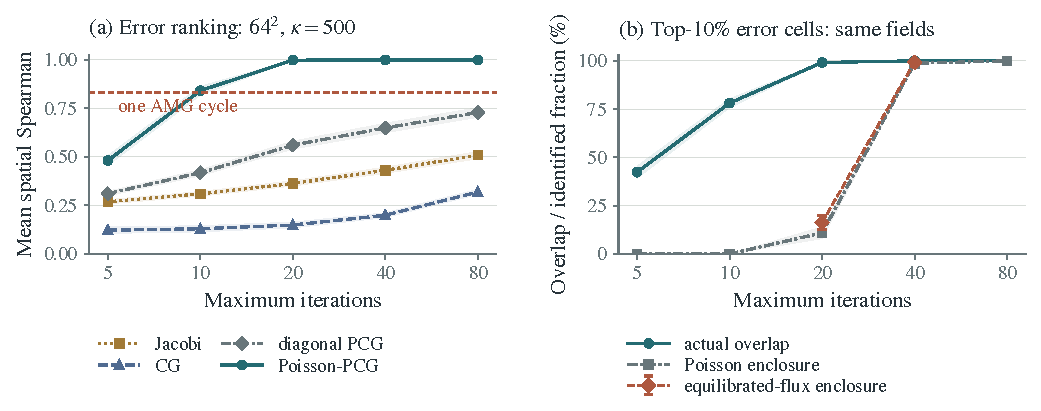
\includegraphics[width=\linewidth]{submission_budget_bounds.pdf}
\caption{Ranking and certification at $64^2$, $\kappa=500$ on fresh binary fields, with $95\%$
field-bootstrap intervals. (a) Rankings improve with budget; AMG uses one cycle. (b) High top-$10\%$
overlap can coexist with few certified members. Flux bounds use $20/40$ iterations. Each bound
evaluation adds one Poisson solve; equal iteration counts are not equal costs.}
\label{fig:budgets}
\end{figure}

\textbf{Accurate rankings can still leave most decisions unresolved.}
At $64^2$, $\kappa=500$, twenty Poisson-PCG steps give a correlation of
$\PoissonLargeFiveHundredPrecise$. The estimated and true top-$10\%$ sets overlap by
$\PoissonTopOverlapPercent\%$ (CI $[\PoissonTopOverlapPercentLow,\PoissonTopOverlapPercentHigh]\%$).
Yet the Poisson bound certifies only $\RecallLargeFiveHundredTwenty\%$ of the true set as members
(CI $[\RecallLargeFiveHundredTwentyLow,\RecallLargeFiveHundredTwentyHigh]\%$).
The flux bound raises this fraction to $\FluxRecallLargeFiveHundredTwenty\%$
(CI $[\FluxRecallLargeFiveHundredTwentyLow,\FluxRecallLargeFiveHundredTwentyHigh]\%$).

With forty iterations, the Poisson bound identifies $\RecallLargeFiveHundredForty\%$ of the true set
(CI $[\RecallLargeFiveHundredFortyLow,\RecallLargeFiveHundredFortyHigh]\%$).
The adaptive rule reaches its $90\%$ target on all $1{,}200$ fresh binary fields. We observe no false
inside/outside flags across the tested fields and budgets. Numerical enclosure checks allow
$10^{-10}\|e\|_\infty+10^{-13}$ floating-point slack; this slack is not added to the bounds used for
decisions.

\textbf{Excellent localization already computes much of the correction.}
Twenty Poisson-PCG steps at $64^2$, $\kappa=500$ leave only
$\PoissonCorrectionRemainingPercent\%$ of the initial error (mean $\|z-e\|_2/\|e\|_2$) and
also supply an improved prediction $\hat u-z$. Assessing the diagnostic must include this correction.

For binary media, we time diagnostics on $30$ fixed fresh fields per setting, using three repetitions, randomized
method order and one Apple M4 CPU thread. At $\kappa=500$, the median paired Poisson-PCG-20/direct-solve
time ratio is $\PoissonTimeLarge$ at $64^2$ (CI $[\PoissonTimeLargeLow,\PoissonTimeLargeHigh]$)
and $\PoissonTimeSmall$ at $32^2$. Given $A$ and $\hat u$, timings include residual formation and
amortize reusable Poisson setup; they do not establish end-to-end speedup. The flux bound reduces
adaptive iterations yet costs $\FluxAdaptiveTimeRatioLarge$ times the original rule at $64^2$:
extra face checks offset the saving.

\section{Discussion and reproducibility}
These discrete results cover one forcing, two modest grids and compact predictors. Continuum
bounds, broader forcing families and universal contrast trends are not established.

Per-field records generate the tables and figures. Checks cover operator identities, independent
inverse calculations, energies, interval separation and frozen-model replay. Codex-assisted code was subject to these checks; scientific design, analysis, and interpretation were author-directed.
The anonymous artifact contains code, seeds, checkpoints and records.

\bibliographystyle{plainnat}
\bibliography{references}
\end{document}
